\documentclass[12pt]{article}

\usepackage[margin=1in]{geometry}	% Narrower margins
\usepackage{booktabs}				% Nice formatting of tables
\usepackage{graphicx}				% Ability to include graphics
\usepackage{hyperref}

\setlength\parindent{0pt}	% Do not indent first line of paragraphs 

% ---- Code listings ----
\usepackage{listings} 					% Nice code layout and inclusion
\usepackage[usenames,dvipsnames]{xcolor}	% Colors (needs to be defined before using colors)

% Define custom colors for listings
\definecolor{listinggray}{gray}{0.98}		% Listings background color
\definecolor{rulegray}{gray}{0.7}			% Listings rule/frame color

% Style for Verilog
\lstdefinestyle{Verilog}{
	language=Verilog,					% Verilog
	backgroundcolor=\color{listinggray},	% light gray background
	rulecolor=\color{blue}, 			% blue frame lines
	frame=tb,							% lines above & below
	linewidth=\columnwidth, 			% set line width
	basicstyle=\small\ttfamily,	% basic font style that is used for the code	
	breaklines=true, 					% allow breaking across columns/pages
	tabsize=3,							% set tab size
	commentstyle=\color{gray},	% comments in italic 
	stringstyle=\upshape,				% strings are printed in normal font
	showspaces=false,					% don't underscore spaces
}

% How to use: \Verilog[listing_options]{file}
\newcommand{\Verilog}[2][]{%
	\lstinputlisting[style=Verilog,#1]{#2}
}



\title{Rotating Square Circuit}
\author{Andrew Clinkenbeard}
\date{\today}

\begin{document}
\maketitle
\section{Introduction}

In this assignment, a rotating square pattern was displayed on a four digit seven segment display. Displayed in the figure below.



\begin{figure}[h]\centering
	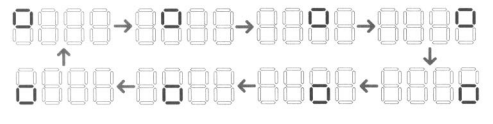
\includegraphics[width=\textwidth,trim=0cm 0cm 0cm 0cm,clip]{figure1}
	\caption{Desired Pattern}
	\label{Desired Pattern}			% label must be after caption
\end{figure}


\section{Method}
\subsection{Counter}
The task was completed by creating a LED time-multiplexing circuit. The code below shows the counter that was used to acomplish the time-mulitplexing. 
\Verilog[firstline=23]{./mysseg.srcs/sources_1/new/counter.sv}
\subsection{Seven Segment Driver}
The counter was then instantiated in a driver for the seven segment displays. This driver used the counter to determine which anode to turn on. The codes is shown below.
\Verilog[firstline=23]{./mysseg.srcs/sources_1/new/ssegdriver.sv}
\subsection{Pattern}
The counter was also instantiated in a module that chooses which step in the pattern the device is currently in. The code is shown below.
\Verilog[firstline=23]{./mysseg.srcs/sources_1/new/Patterns.sv}
\subsection{Main}
Finally the above modules were instantiated in a top level module which connected the modules together to enable the pattern to show up on the physical hardware. The code is shown below.
\Verilog[firstline=23]{./mysseg.srcs/sources_1/new/ssegmain.sv}

\section{Testing}
An expected error was the pattern moving counter-clockwise instead clock-wise. The fix for this was to reverse the order in the Patterns file of which patter appeared when.
Another expected error was to have inccorect timing. This would have caused the LEDs to not turn on and off fast enough to be seen as continuous by humans.


\section{Results}
The pattern matched the intdeded result. The square was able to rotate around the display.

\section{Conclusion}
In conclusion, the pattern was displayed as wanted. The seven segment displays were used as expected. The resulting pattern can be seen at this \href{https://www.youtube.com/watch?v=FZpEwH8YCFI}{link}.


\end{document}